%iffalse
\let\negmedspace\undefined
\let\negthickspace\undefined
\documentclass[journal,12pt,onecolumn]{IEEEtran}
\usepackage{cite}
\usepackage{amsmath,amssymb,amsfonts,amsthm}
\usepackage{algorithmic}
\usepackage{graphicx}
\usepackage{textcomp}
\usepackage{xcolor}
\usepackage{txfonts}
\usepackage{listings}
\usepackage{enumitem}
\usepackage{mathtools}
\usepackage{gensymb}
\usepackage{comment}
\usepackage[breaklinks=true]{hyperref}
\usepackage{tkz-euclide} 
\usepackage{listings}
\usepackage{gvv}                                        
% \usepackage{gvv}  
\usepackage[latin1] {inputenc}
\usepackage{xparse}
\usepackage{color}                                            
\usepackage{array}                                            
\usepackage{longtable}                                       
\usepackage{calc}                                             
\usepackage{multirow}
\usepackage{multicol}
\usepackage{hhline}                                           
\usepackage{ifthen}                                           
\usepackage{lscape}
\usepackage{tabularx}
\usepackage{array}
\usepackage{float}
\newtheorem{theorem}{Theorem}[section]
\newtheorem{problem}{Problem}
\newtheorem{proposition}{Proposition}[section]
\newtheorem{lemma}{Lemma}[section]
\newtheorem{corollary}[theorem]{Corollary}
\newtheorem{example}{Example}[section]
\newtheorem{definition}[problem]{Definition}
\newcommand{\BEQA}{\begin{eqnarray}}
\newcommand{\EEQA}{\end{eqnarray}}
\usepackage{float}
%\newcommand{\define}{\stackrel{\triangle}{=}}
\theoremstyle{remark}
\usepackage{ circuitikz }
%\newtheorem{rem}{Remark}
% Marks the beginning of the document
\begin{document}
\title{GATE BT 2013}
\author{EE25BTECH11044 - Pappula Sai Hasini}
\maketitle
\renewcommand{\thefigure}{\theenumi}
\renewcommand{\thetable}{\theenumi}
%GATE BT 2013
\begin{enumerate}
    \item 


Under alkaline conditions, DNA is more stable than RNA because:

\begin{enumerate}
    \item RNA forms secondary structures
    \item RNA is a single stranded molecule
    \item RNA has uracil in place of thymidine
    \item RNA is susceptible to hydrolysis
\end{enumerate} 
\hfill (GATE BT 2013)

\item Which one of the following modifications is common to both protein and DNA?

\begin{enumerate}
    \item Sumoylation
    \item Nitrosylation
    \item Methylation
    \item Ubiquitination
\end{enumerate} 
\hfill (GATE BT 2013)

\item Protein A, which has strong affinity to Fc region of immunoglobulin, is extracted from:

\begin{enumerate}
    \item \textit{Saccharomyces cerevisiae}
    \item \textit{Staphylococcus aureus}
    \item \textit{Streptococcus pyogenes}
    \item \textit{Streptococcus sanguis}
\end{enumerate}
\hfill (GATE BT 2013)

\item The first humanized monoclonal antibody approved for the treatment of breast cancer is:

\begin{enumerate}
    \item Rituximab
    \item Cetuximab
    \item Bevacizumab
    \item Herceptin
\end{enumerate} 
\hfill (GATE BT 2013)

\item Which one of the following amino acids in proteins does \textbf{NOT} undergo phosphorylation?

\begin{enumerate}
    \item Ser 
    \item Thr
    \item Pro
    \item Tyr
\end{enumerate} 
\hfill (GATE BT 2013)

\item 

The role of an adjuvant is to: 

\begin{enumerate}
    
    \item Prolong the persistence of antigen
    \item Cross link the antigen
    \item Increase the size of antigen
    \item Avoid inflammation
\end{enumerate} 
\hfill (GATE BT 2013)

\item

Endogenous antigens are presented on to the cell surface along with:

\begin{enumerate}
    \item MHC-II
    \item MHC-I
    \item Fc$\gamma$ receptor
    \item Complement receptor
\end{enumerate} 
\hfill (GATE BT 2013)
\item

Human genome sequencing project involved the construction of genomic library in:

\begin{enumerate}
    \item Bacterial artificial chromosome
    \item pBR322
    \item Bacteriophage
    \item pcDNA3.1
\end{enumerate} 
\hfill (GATE BT 2013)
\item 

The nucleotide analogue used in DNA sequencing by chain termination method is:

\begin{enumerate}
    \item 1',3'-dideoxy nucleoside triphosphate
    \item 2',3'-dideoxy nucleoside triphosphate
    \item 2',4'-dideoxy nucleoside triphosphate
    \item 2',5'-dideoxy nucleoside triphosphate
\end{enumerate}
\hfill (GATE BT 2013)
\item 

In nature, the horizontal gene transfer across bacteria is mediated by:

\begin{enumerate}
    \item Gene cloning followed by transformation
    \item Conjugation and transformation
    \item Conjugation only
    \item Transformation only
\end{enumerate} 
\hfill (GATE BT 2013)
\item 

Phylum proteobacteria is subdivided into $\alpha$-, $\beta$-, $\gamma$-, $\delta$- and $\varepsilon$-proteobacteria based on:

\begin{enumerate}
    \item G+C content
    \item 23S rRNA sequences
    \item tRNA sequences
    \item 16S rRNA sequences
\end{enumerate}
\hfill (GATE BT 2013)
\item 

Which one of the following is an ABC transporter?

\begin{enumerate}
    \item Multidrug resistance protien 
    \item Acetylcholine receptor
    \item Bacteriorhodopsin
    \item ATP synthase
\end{enumerate} 
\hfill (GATE BT 2013)
\item 

The catalytic efficiency for an enzyme is defined as:

\begin{enumerate}
    \item $k_{cat}$
    \item $\dfrac{V_{max}}{k_{cat}}$
    \item {$\dfrac{k_{cat}}{K_m}$} 
    \item $\dfrac{k_{cat}}{V_{max}}$
\end{enumerate} 
\hfill (GATE BT 2013)
\item 

Of the two diploid species, species I has 36 chromosomes and species II has 28 chromosomes. How many chromosomes would be found in an allotriploid individual?

\begin{enumerate}
    \item $42$ or $54$
    \item $46$ or $50$
    \item $74$ or $86$
    \item $84$ or $108$
\end{enumerate} 
\hfill (GATE BT 2013)
\item 

The RNA primer synthesized during the replication process in bacteria is removed by:

\begin{enumerate}
    \item DNA gyrase
    \item Primase
    \item DNA polymerase I
    \item DNA polymerase II
\end{enumerate} 
\hfill (GATE BT 2013)
\item 

The suitable substitution matrix to align closely related sequences is:

\begin{enumerate}
    \item PAM $250$ or BLOSUM $80$
    \item PAM $40$ or BLOSUM $80$
    \item PAM $120$ or BLOSUM $40$
    \item PAM $250$ or BLOSUM $40$
\end{enumerate} 
\hfill (GATE BT 2013)
\item 

If 
\[
\vec{P} = \begin{bmatrix}
1 & 1 \\
2 & 2
\end{bmatrix},
\quad
\vec{Q} = \begin{bmatrix}
1 & 2 \\
2 & 2
\end{bmatrix},
\quad
\vec{R} = \begin{bmatrix}
0 & 3 \\
3 & 1
\end{bmatrix}
\]

which one of the following statements is TRUE?

\begin{enumerate}
    \item $PQ = PR$
    \item $QR = RP$
    \item $QP = RP$
    \item $PQ = QR$
\end{enumerate}
\hfill (GATE BT 2013)
\item 

If \( u = \log \left( e^{x} + e^{y} \right) \), then find \( \frac{du}{dx} + \frac{du}{dy} \):

\begin{enumerate}
    \item $e^{x} + e^{y}$
    \item $e^{x} - e^{y}$
    \item\( \frac{1}{e^x + e^y} \)
    \item 1
\end{enumerate} 
\hfill (GATE BT 2013)
\item 

Hypophosphatemia is manifested by an X-linked dominant allele. What proportion of the offspring from a normal male and an affected heterozygous female will manifest the disease?

\begin{enumerate}
    \item $\frac{1}{2}$ sons and $\frac{1}{2}$ daughters
    \item All daughters and no sons
    \item All sons and no daughters
    \item $\frac{1}{4}$ daughters and $\frac{1}{4}$ sons
\end{enumerate} 
\hfill (GATE BT 2013)
\item 

One of the eigenvalues of 
\[
\vec{P} = \left[
\begin{array}{cc}
10 & -18 \\
4 & -12
\end{array}
\right]
\]
is:

\begin{enumerate}
    \item $2$
    \item $4$
    \item $6$
    \item $8$
\end{enumerate} 
\hfill (GATE BT 2013)
\item 

A callus of 5 g dry weight was inoculated on semi-solid medium for growth. The dry weight of the callus was found to increase by 1.5 fold after 10 days of inoculation. The growth index of the culture is \_.
\hfill (GATE BT 2013)
\item 

A chemostat is operated at a dilution rate of 0.6 h$^{-1}$. At steady state, the biomass concentration in the exit stream was found to be 30 g L$^{-1}$. The biomass productivity (g L$^{-1}$ h$^{-1}$) after 3 h of steady state operation will be \_\_\_\_\_\_\_.
\hfill (GATE BT 2013)

\item 

A batch bioreactor is to be scaled up from 10 to 10,000 liters. The diameter of the large bioreactor is 10 times that of the small bioreactor. The agitator speed in the small bioreactor is 450 rpm. Determine the agitator speed (rpm) of the large bioreactor with the same impeller tip speed as that of the small bioreactor. \_\_\_\_\_\_\_.
\hfill (GATE BT 2013)
\item 

Calculate the percentage sequence identity for the pairwise alignment given below. \_\_\_\_\_\_\_
\hfill (GATE BT 2013)
\item 

In a batch culture, the specific rate of substrate utilization is 0.25 g (g cell mass)$^{-1}$ h$^{-1}$ and specific rate of product formation is 0.215 g (g cell mass)$^{-1}$ h$^{-1}$. Calculate the yield of product from the substrate (Y$_{p/s}$). \_\_\_\_\_\_\_.
\hfill (GATE BT 2013)
\item 

Match the commercial microbial sources in Group I with the products in Group II.

\begin{tabbing}
Group I \hspace{3cm} \= Group II \\
P. Corynebacterium \textit{lilium} \> 1. 2,3-Butane di-ol \\
Q. Klebsiella \textit{oxytoca} \> 2. Poly-$\beta$-hydroxybutyric acid \\
R. \textit{Aspergillus niger} \> 3. Glutamic acid \\
S. \textit{Alcaligenes eutrophus} \> 4. Citric acid \\
\end{tabbing}

\begin{enumerate}
    \item P-3, Q-1, R-2, S-4
    \item P-3, Q-1, R-4, S-2
    \item P-1, Q-3, R-2, S-4
    \item P-1, Q-3, R-4, S-2
\end{enumerate} 
\hfill (GATE BT 2013)
\item 

Match the entries in Group I with the elution conditions in Group II.

\begin{tabbing}
Group I \hspace{6cm} \= Group II \\
P. Ion-exchange chromatography \> 1. Isocratic solvent \\
Q. Hydrophobic column chromatography \> 2. Ampholytes \\
R. Gel filtration chromatography \> 3. Increasing gradient of salt \\
S. Chromatofocusing \> 4. Decreasing gradient of polarity \\
\end{tabbing}

\begin{enumerate}
    \item P-4, Q-1, R-2, S-3
    \item P-4, Q-3, R-1, S-2
    \item P-3, Q-4, R-1, S-2
    \item P-3, Q-4, R-2, S-1
\end{enumerate} 
\hfill (GATE BT 2013)
\item 

Determine the correctness or otherwise of the following Assertion (a) and Reason (r).

\textbf{Assertion (a):} Immobilization of plant cells can enhance secondary metabolite production during bioreactor cultivation.

\textbf{Reason (r):} Immobilization protects the plant cells from shear forces in the bioreactor.

\begin{enumerate}
    \item Both (a) and (r) are true and (r) is the correct reason for (a).
    \item Both (a) and (r) are true but (r) is not the correct reason for (a).
    \item (a) is true but (r) is false.
    \item (a) is false but (r) is true.
\end{enumerate} 
\hfill (GATE BT 2013)
\item 

Match the cell structures in Group I with the organisms in Group II.

\begin{tabbing}
Group I \hspace{3.5cm} \= Group II \\
P. Endospores \> 1. \textit{Methanobacterium} \\
Q. Bipolar flagella \> 2. \textit{Treponema} \\
R. Pseudomurine in cell wall \> 3. \textit{Spirillum} \\
S. Periplasmic flagella \> 4. \textit{Clostridium} \\
\end{tabbing}

\begin{enumerate}
    \item P-4, Q-3, R-1, S-2
    \item P-4, Q-3, R-2, S-1
    \item P-3, Q-4, R-1, S-2
    \item P-4, Q-1, R-3, S-2
\end{enumerate} 
\hfill (GATE BT 2013)
\item 

Match the antibiotics in Group I with the targets in Group II.

\begin{tabbing}
Group I \hspace{3.5cm} \= Group II \\
P. Sulfonamide \> 1. Peptidoglycan synthesis \\
Q. Quinolones \> 2. Peptide chain elongation \\
R. Erythromycin \> 3. Folic acid biosynthesis \\
S. Cephalosporin \> 4. Topoisomerase \\
\end{tabbing}

\begin{enumerate}
    \item P-3, Q-4, R-1, S-2
    \item P-2, Q-4, R-3, S-1
    \item P-4, Q-1, R-2, S-3
    \item P-3, Q-4, R-2, S-1
\end{enumerate} \hfill(GATE BT 2013)

\item 

In nature, \textit{Agrobacterium tumefaciens} mediated infection of plant cells leads to:

\begin{enumerate}
    \item S only
    \item P and R only
    \item Q and S only
    \item Q only
\end{enumerate} \hfill(GATE BT 2013)

Where:  
P. Crown gall disease in plants  
Q. Hairy root disease in plants  
R. Transfer of T-DNA into the plant chromosome  
S. Transfer of Ri-plasmid into the plant cell
\item 

Match the entries in Group I with the enzymes in Group II.

\begin{tabbing}
Group I \hspace{3.5cm} \= Group II \\
P. NAD$^+$ \> 1. Glutathione peroxidase \\
Q. Selenium \> 2. Nitrogenase \\
R. Pyridoxal phosphate \> 3. Lactate dehydrogenase \\
S. Molybdenum \> 4. Glycogen phosphorylase \\
\end{tabbing}

\begin{enumerate}
    \item P-3, Q-2, R-4, S-1
    \item P-4, Q-1, R-3, S-2
    \item P-3, Q-1, R-4, S-2
    \item P-3, Q-4, R-2, S-1
\end{enumerate} \hfill(GATE BT 2013)

\item 

Match the herbicides in Group I with the target enzymes in Group II.

\begin{tabbing}
Group I \hspace{3.5cm} \= Group II \\
P. Glyphosate \> 1. Nitrilase \\
Q. Bromoxynil \> 2. Acetolactate synthetase \\
R. Sulphonylureas \> 3. Dehalogenase \\
S. Dalapon \> 4. 5-Enolpyruvyl shikimate-3-phosphate synthase \\
\end{tabbing}


  \item The activity of an enzyme was measured by varying the concentration of the substrate (S) 
    in the presence of three different concentrations of inhibitor (I) 0, 2 and 4 mM. 
    The double reciprocal plot given below suggests that the inhibitor (I) exhibits

\begin{figure}[htbp]
  \centering
  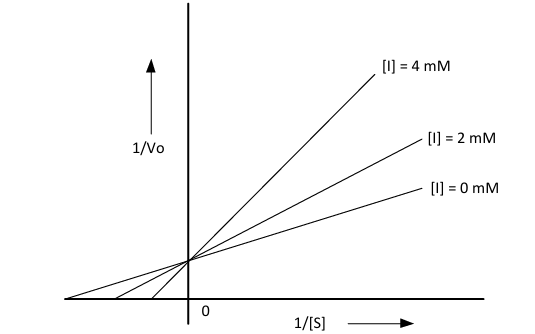
\includegraphics[width=\columnwidth]{figs/enzyme_plot.png}
  \caption{Double reciprocal plot of enzyme activity with different inhibitor concentrations}
  \label{fig:enzyme_plot}
\end{figure}

\begin{enumerate}
    \item[(A)] substrate inhibition
    \item[(B)] uncompetitive inhibition
    \item[(C)] mixed inhibition
    \item[(D)] competitive inhibition
\end{enumerate} \hfill(GATE BT 2013)


\begin{enumerate}
    \item P-4, Q-1, R-2, S-3
    \item P-2, Q-1, R-4, S-3
    \item P-4, Q-3, R-2, S-1
    \item P-3, Q-2, R-4, S-1
\end{enumerate} \hfill(GATE BT 2013)


\item 

Match the entries in Group I with the entries in Group II.

\begin{tabbing}
Group I \hspace{3.5cm} \= Group II \\
P. RNase P \> 1. Polyadenylation \\
Q. RNase H \> 2. Splicing \\
R. snRNAs \> 3. Ribozymes \\
S. CstF \> 4. DNA-RNA hybrids \\
\end{tabbing}

\begin{enumerate}
    \item P-3, Q-4, R-2, S-1
    \item P-4, Q-3, R-2, S-1
    \item P-3, Q-2, R-1, S-4
    \item P-2, Q-4, R-1, S-3
\end{enumerate} \hfill(GATE BT 2013)

\item 

Determine the correctness or otherwise of the following Assertion (a) and Reason (r).

\textbf{Assertion (a):} UPGMA method produces an ultrametric tree.

\textbf{Reason (r):} Sequence alignment is converted into evolutionary distances in the UPGMA method.

\begin{enumerate}
    \item Both (a) and (r) are true and (r) is the correct reason for (a)
    \item Both (a) and (r) are true but (r) is not the correct reason for (a)
    \item (a) is true but (r) is false
    \item (a) is false but (r) is true
\end{enumerate} \hfill(GATE BT 2013)

\item 

Match the entries in Group I with the entries in Group II.

\begin{tabbing}
Group I \hspace{3.5cm} \= Group II \\
P. Threading \> 1. Gene duplication \\
Q. FASTA \> 2. Fold prediction \\
R. Profile \> 3. HMM \\
S. Paralogs \> 4. k-tuple \\
\end{tabbing}

\begin{enumerate}
    \item P-2, Q-1, R-3, S-4
    \item P-2, Q-4, R-3, S-1
    \item P-3, Q-4, R-2, S-1
    \item P-1, Q-4, R-3, S-2
\end{enumerate} \hfill(GATE BT 2013)

\item 

Evaluate \(\displaystyle \lim_{x \to \infty} \frac{\tan x}{x}\).

\begin{enumerate}
    \item \(\infty\)
    \item $1$
    \item $0$
    \item $-1$
\end{enumerate} \hfill(GATE BT 2013)

\item 

The Laplace transform of f(t)=2t + 6 is 

\begin{enumerate}
    \item 1/s + \( \frac{2}{s^2} \)
    \item 3/s - \(\frac{6}{s^2}\)
    \item 6/s + \(\frac{2}{s^2}\)
    \item -6/s +\(\frac{2}{s^2}\)

\end{enumerate} \hfill(GATE BT 2013)

\item 

The solution of the following set of equations is:
\[
\begin{aligned}
2x + 3y + z &= 20 \\
7x + 3y + z &= 13 \\
6x + 2y + z &= 0
\end{aligned}
\]

\begin{enumerate}
    \item $2,\ 2,\ 8$
    \item $2,\ 3,\ 8$
    \item $2,\ 3,\ 8$
    \item $8,\ 2,\ 3$
\end{enumerate} \hfill(GATE BT 2013)

\item 

The solution to the differential equation 
\[
\frac{dy}{dx} + y \cot x = \csc x
\]
is:

\begin{enumerate}
    \item \( y = (c + x) \cot x \)
    \item \( y = (c + x) \csc x \)
    \item \( y = (c + x) \csc x \cot x \)
    \item \( y = \frac{(c + x) \csc x}{\cot x} \)
\end{enumerate} \hfill(GATE BT 2013)

\item 

A complete restriction digestion of a circular plasmid (5000 bp) was carried out with HindIII, BamHI, and EcoRI individually. Restriction digestion yielded the following fragments:

\[
\begin{aligned}
\text{Plasmid + HindIII} &\to 1200 \text{ bp and } 3800 \text{ bp} \\
\text{Plasmid + BamHI} &\to 5000 \text{ bp} \\
\text{Plasmid + EcoRI} &\to 2500 \text{ bp}
\end{aligned}
\]

The number of sites for EcoRI, BamHI, and HindIII present on this plasmid are:

\begin{enumerate}
    \item EcoRI - 2, BamHI - 1, HindIII - 2
    \item EcoRI - 1, BamHI - 1, HindIII - 2
    \item EcoRI - 3, BamHI - 2, HindIII - 1
    \item EcoRI - 2, BamHI - 2, HindIII - 1
\end{enumerate} \hfill(GATE BT 2013)

\item 

The total number of fragments generated by the complete and sequential cleavage of the polypeptide given below by Trypsin followed by CNBr is \_\_\_\_\_\_\_.

\[
\text{Phe-Trp-Met-Gly-Ala-Lys-Leu-Pro-Met-Asp-Gly-Arg-Cys-Ala-Gln}
\]
\item 

In a genetic study, 80 people were found to have alleles for polydactyly. Only 36 of them were polydactylous. What is the extent of penetrance percentage? \_\_\_\_\_\_\_

\item 

One percent of the cars manufactured by a company are defective. What is the probability (up to four decimals) that more than two cars are defective, if 100 cars are produced? \_\_\_\_\_\_\_

\item 

The maximum cell concentration (g\,l\(^{-1}\)) expected in a bioreactor with initial cell concentration of 1.75 g\,l\(^{-1}\) and an initial glucose concentration of 125 g\,l\(^{-1}\) is \(\left(Y_{x/s} = 0.6 \text{ g cell/g substrate}\right)\) \_\_\_\_\_\_\_

\item 

A fed batch culture was operated with intermittent addition of glucose solution at a flow rate of 200 ml h\(^{-1}\). The values of \(K_s\), \(\mu_m\), and \(D\) are 0.3 g\,l\(^{-1}\), 0.4 h\(^{-1}\), and 0.1 h\(^{-1}\), respectively. Determine the concentration of growth limiting substrate (g\,l\(^{-1}\)) in the reactor at quasi-steady state. \_\_\_\_\_\_\_
\item 

A solution was prepared by dissolving 100 mg of protein X in 100 ml of water.  
Molecular weight of protein \(X\) is \(15{,}000\ \mathrm{Da};\) Avogadro's number \(= 6.022 \times 10^{23}\)

Calculate the molarity (\(\mu M\)) of the resulting solution.

\begin{enumerate}
    \item $66.6$
    \item $6.6$
    \item $0.67$
    \item $0.067$
\end{enumerate} \hfill(GATE BT 2013)

\item 

The number of molecules present in this solution is:

\begin{enumerate}
    \item $40.15 \times 10^{19}$
    \item $6.023 \times 10^{19}$
    \item $4.015 \times 10^{19}$
    \item $0.08 \times 10^{19}$
\end{enumerate} \hfill(GATE BT 2013)

\item 
The binding efficiency of three different receptors R1, R2 and R3 were tested against a ligand using 
equilibrium dialysis, with a constant concentration of receptor and varying concentrations of ligand. 
The Scatchard plot of receptor titration with different concentrations of ligand is given below 
(\(r\) is moles of bound ligand per moles of receptor and \(c\) is concentration of free ligand).

\begin{figure}[htbp]
  \centering
  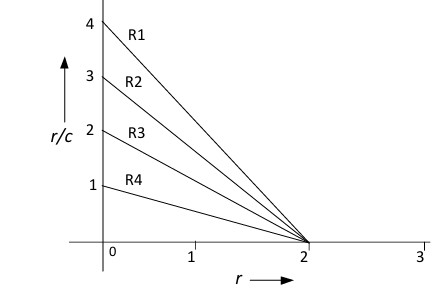
\includegraphics[width=\columnwidth]{figs/scatchard_plot.png}
  \caption{Scatchard plot of receptor titration with ligand concentration}
  \label{fig:scatchard_plot}
\end{figure}

\begin{enumerate}
    \item The number of ligand binding sites present on receptors R1 and R3, respectively, are:
    \begin{enumerate}
        \item[(A)] 1 and 4
        \item[(B)] 1 and 1
        \item[(C)] 4 and 1
    \end{enumerate} \hfill(GATE BT 2013)
\end{enumerate}

    \item Which one of the receptors has the highest affinity for the ligand?
    \begin{enumerate}
        \item[(A)] R1
        \item[(B)] R2
        \item[(C)] R3
        \item[(D)] R4
    \end{enumerate} \hfill(GATE BT 2013)


\item 
A DNA fragment of 5000 bp needs to be isolated from \textit{E.~coli} (genome size \(4 \times 10^{3}\) kb) genomic library.

    The minimum number of independent recombinant clones required to represent this fragment in the genomic library are:

\begin{enumerate}
    \item \(16 \times 10^{2}\)
    \item \(12 \times 10^{2}\)
    \item \(8 \times 10^{2}\)
    \item \(1.25 \times 10^{2}\)
\end{enumerate} \hfill(GATE BT 2013)

\item 

The number of clones to represent this fragment in the genomic library with a probability of 95% are:

\begin{enumerate}
    \item \(5.9 \times 10^{3}\)
    \item \(4.5 \times 10^{3}\)
    \item \(3.6 \times 10^{3}\)
    \item \(2.4 \times 10^{3}\)
\end{enumerate} \hfill(GATE BT 2013)

\item 

During sterilization of a fermentation medium in a given bioreactor, \(\Delta_{\text{heating}} = 12.56\), \(\Delta_{\text{cooling}} = 7.48\), and the total value of \(\Delta\) required for the whole sterilization process is 52, where \(\Delta\) is the design criteria.

What is the value of \(\Delta_{\text{holding}}\)?

\begin{enumerate}
    \item $31.96$
    \item $42.32$
    \item $52.43$
\end{enumerate} \hfill(GATE BT 2013)

\item 

What is the holding period (min) at a \(k\) value of \(3.36 \text{ min}^{-1}\)?

\begin{enumerate}
    \item $10.6$
    \item $9.5$
    \item $8.4$
    \item $61.18$
    \item $7.2$
\end{enumerate} \hfill(GATE BT 2013)

\item 
If \(3 \le X \le 5\) and \(8 \le Y \le 11\) then which of the following options is \textbf{TRUE}?

\begin{enumerate}
    \item[(A)] \(\frac{3}{5} \le \frac{X}{Y} \le \frac{8}{5}\)
    \item[(B)] \(\frac{3}{11} \le \frac{X}{Y} \le \frac{5}{8}\)
    \item[(C)] \(\frac{3}{11} \le \frac{X}{Y} \le \frac{8}{5}\)
    \item[(D)] \(\frac{3}{5} \le \frac{X}{Y} \le \frac{8}{11}\)
\end{enumerate} \hfill(GATE BT 2013)

\item 

The Headmaster \_\_\_\_\_\_\_\_\_ to speak to you. 

Which of the following options is incorrect to complete the above sentence?

\begin{enumerate}
    \item is wanting
    \item wants
    \item want
    \item was wanting
\end{enumerate} \hfill(GATE BT 2013)

\item 

Mahatma Gandhi was known for his humility as

\begin{enumerate}
    \item he played an important role in humiliating exit of British from India.
    \item he worked for humanitarian causes.
    \item he displayed modesty in his interactions.
    \item he was a fine human being.
\end{enumerate} \hfill(GATE BT 2013)

\item 

All engineering students should learn mechanics, mathematics and how to do computation.

\[
\underbrace{\text{All engineering students}}_{I} \quad
\underbrace{\text{should learn mechanics}}_{II} \quad
\underbrace{\text{mathematics}}_{III} \quad
\underbrace{\text{and how to do computation}}_{IV}
\]

Which of the above underlined parts of the sentence is not appropriate?

\begin{enumerate}
    \item I
    \item II
    \item III
    \item IV
\end{enumerate} \hfill(GATE BT 2013)

\item 

Select the pair that best expresses a relationship similar to that expressed in the pair:  
water : pipe ::

\begin{enumerate}
    \item cart : road
    \item electricity : wire
    \item sea : beach
    \item music : instrument
\end{enumerate} \hfill(GATE BT 2013)

\item 

Velocity of an object fired directly in upward direction is given by
\[
V = 80 - 32t,
\]
where time \(t\) is in seconds. When will the velocity be between 32 m/sec and 64 m/sec?

\begin{enumerate}
    \item \((1, \tfrac{3}{2})\)
    \item \(\left(\tfrac{1}{2}, 1\right)\)
    \item \(\left(\tfrac{1}{2}, \tfrac{3}{2}\right)\)
    \item \((1, 3)\)
\end{enumerate} \hfill(GATE BT 2013)

\item 

In a factory, two machines M1 and M2 manufacture 60\% and 40\% of the autocomponents respectively. Out of the total production, 2\% of M1 and 3\% of M2 are found to be defective. If a randomly drawn autocomponent from the combined lot is found defective, what is the probability that it was manufactured by M2?

\begin{enumerate}
    \item $0.35$
    \item $0.45$
    \item $0.5$
    \item $0.4$
\end{enumerate} \hfill(GATE BT 2013)

\item 
Following table gives data on tourists from different countries visiting India in the year 2011.

\begin{center}
\begin{tabular}{|c|c|}
\hline
\textbf{Country} & \textbf{Number of Tourists} \\
\hline
USA & 2000 \\
England & 3500 \\
Germany & 1200 \\
Italy & 1100 \\
Japan & 2400 \\
Australia & 2300 \\
France & 1000 \\
\hline
\end{tabular}
\end{center}

Which two countries contributed to one-third of the total number of tourists who visited India in 2011?

\begin{enumerate}
    \item[(A)] USA and Japan
    \item[(B)] USA and Australia
    \item[(C)] England and France
    \item[(D)] Japan and Australia
\end{enumerate} \hfill(GATE BT 2013)

\item 

If \(\left| -2X + 9 \right| = 3\), then the possible value of \(\left| -X \right| - X^2\) would be:

\begin{enumerate}
    \item $30$
    \item $-30$
    \item $42$
    \item $-42$
\end{enumerate} \hfill(GATE BT 2013)

\item 
All professors are researchers. \\
Some scientists are professors. \\

Which of the given conclusions is logically valid and is inferred from the above arguments?

\begin{enumerate}
    \item All scientists are researchers
    \item All professors are scientists
    \item Some researchers are scientists
    \item No conclusion follows
\end{enumerate} \hfill(GATE BT 2013)
\end{enumerate}
\end{document}




